\documentclass[ignorenonframetext,aspectratio=169]{beamer}

\usetheme[]{rli}

\tikzset{
invisible/.style={opacity=0},
visible on/.style={alt={#1{}{invisible}}},
alt/.code args={<#1>#2#3}{%
  \alt<#1>{\pgfkeysalso{#2}}{\pgfkeysalso{#3}} % \pgfkeysalso doesn't change the path
},
}

\title{The RLI \LaTeX{} beamer theme}
\subtitle{\ldots finally overcoming MS Powerpoint}
\author{Guido Pleßmann \and Jann Launer \and Matthias Laugwitz}
\date{\today}
\institute{Reiner Lemoine Institut}

\newcommand{\tel}{+49 (0)30 1208 434 72}
\newcommand{\email}{guido.plessmann@rl-institut.de}
\newcommand{\twitter}{\href{https://twitter.com/gplssm}{@gplssm}}
\newcommand{\finalstatement}{Enjoy stating a final statement ;-)}

\begin{document}
\frame{\titlepage}

\begin{frame}[fragile]{A new frame}
Create a new frame with title and content
\end{frame}

% \begin{frame}[fragile]{Use formatting syntax}
% \protect\hypertarget{use-formatting-syntax}{}

% The \emph{quick} \textbf{brown} fox \textsuperscript{jumps}
% \textsubscript{over} the \texttt{lazy} \texttt{dog}\sout{, not the cat}.

% You can also quote it

% \begin{quote}
% The quick brown fox jumps over the lazy dog, not the cat.
% \end{quote}

% Moreover, you can simply write \LaTeX{} code in .md files.

% \end{frame}

% \begin{frame}{Use lists and enumerated lists}
% \protect\hypertarget{use-lists-and-enumerated-lists}{}

% \begin{itemize}
% \tightlist
% \item
%   item a

%   \begin{itemize}
%   \tightlist
%   \item
%     item a.1

%     \begin{itemize}
%     \tightlist
%     \item
%       item a.1.a
%     \item
%       item a.1.b
%     \end{itemize}
%   \end{itemize}
% \end{itemize}

% \begin{enumerate}
% \tightlist
% \item
%   item 1

%   \begin{enumerate}
%   \tightlist
%   \item
%     item a
%   \end{enumerate}
% \item
%   item 2
% \item
%   item 3

%   \begin{itemize}
%   \tightlist
%   \item
%     mix
%   \item
%     it
%   \end{itemize}
% \end{enumerate}

% \end{frame}

% \begin{frame}{Descriptions}
% \protect\hypertarget{descriptions}{}

% \begin{description}
% \tightlist
% \item[Distributed Energy Resource]
% Electrical power generation or storage located at or near the point of
% use, as well as demand side measures.
% \item[Distributed Generation]
% Electric power generation located at or near the point of use.
% \item[Distributed Power]
% Electrical power generation or storage located at or near the point of
% use.
% \end{description}

% \footnotesize Content stolen from
% \href{https://aceee.org/glossary_data}{ACEEE glosarry}.

% \end{frame}

% \begin{frame}{Insert images}
% \protect\hypertarget{insert-images}{}

% \center

% 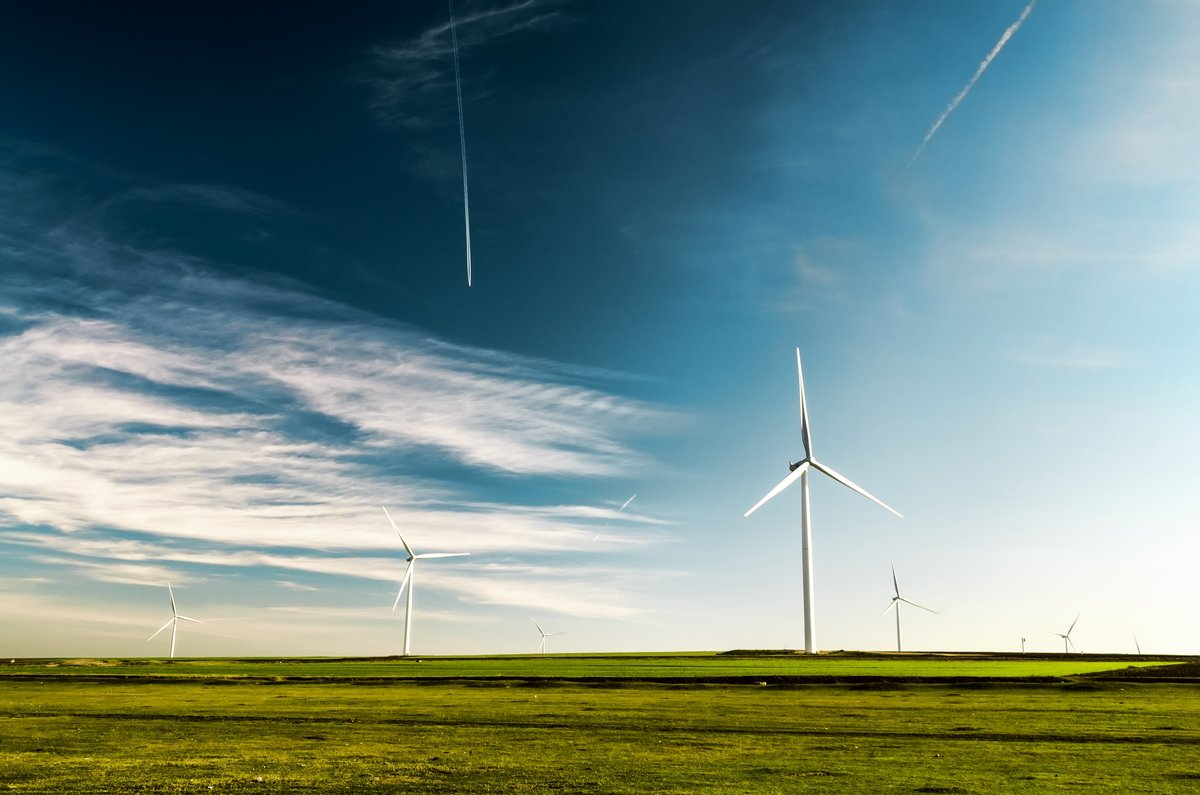
\includegraphics[width=0.75\textwidth,height=\textheight]{img/createria-ZYu6P9-Glic-unsplash_resized.jpg}

% \end{frame}

% \begin{frame}[fragile]{Presenting code}
% \protect\hypertarget{presenting-code}{}

% \begin{Shaded}
% \begin{Highlighting}[]
% \ImportTok{import}\NormalTok{ requests}
% \ImportTok{import}\NormalTok{ pandas }\ImportTok{as}\NormalTok{ pd}
% \ImportTok{from}\NormalTok{ tabulate }\ImportTok{import}\NormalTok{ tabulate}

% \NormalTok{df }\OperatorTok{=}\NormalTok{ pd.DataFrame(requests.get(}\StringTok{'http://openenergy-platform.org/api/v0\textbackslash{}}
% \StringTok{  /schema/supply/tables/bnetza_eeg_anlagenstammdaten/rows/?limit=100'}\NormalTok{).json())}

% \NormalTok{df }\OperatorTok{=}\NormalTok{ df[[}
%   \StringTok{'4.11_bundesland'}\NormalTok{,}
%   \StringTok{'4.1_energieträger'}\NormalTok{, }
%   \StringTok{'4.2_installierte_leistung'}\NormalTok{,}
%   \StringTok{'4.16_name_des_netzbetreibers'}\NormalTok{]]}
% \NormalTok{df.columns }\OperatorTok{=}\NormalTok{ [}\StringTok{"Federal state"}\NormalTok{, }\StringTok{"Technology"}\NormalTok{, }\StringTok{"Inst. Power"}\NormalTok{, }\StringTok{"Grid operator"}\NormalTok{]}

% \BuiltInTok{print}\NormalTok{(tabulate(df.head(}\DecValTok{10}\NormalTok{), tablefmt}\OperatorTok{=}\StringTok{"pipe"}\NormalTok{, headers}\OperatorTok{=}\StringTok{"keys"}\NormalTok{))}
% \end{Highlighting}
% \end{Shaded}

% \end{frame}

% \begin{frame}{Tables}
% \protect\hypertarget{tables}{}

% \begin{longtable}[]{@{}rllrl@{}}
% \toprule
% & Federal state & Technology & Inst. Power & Grid
% operator\tabularnewline
% \midrule
% \endhead
% 0 & Niedersachsen & Biomasse & 366 & Avacon AG\tabularnewline
% 1 & Bayern & Biomasse & 380 & Bayernwerk AG\tabularnewline
% 2 & Bayern & Wasserkraft & 6 & Bayernwerk AG\tabularnewline
% 3 & Hessen & Biomasse & 380 & EnergieNetz Mitte GmbH\tabularnewline
% 4 & Bayern & Wind Land & 3050 & Bayernwerk AG\tabularnewline
% 5 & Nordrhein-Westfalen & Biomasse & 400 & Westfalen Weser Netz
% GmbH\tabularnewline
% 6 & Nordrhein-Westfalen & Biomasse & 1200 & Westfalen Weser Netz
% GmbH\tabularnewline
% 7 & Schleswig-Holstein & Wind Land & 2000 & Schleswig-Holstein Netz
% AG\tabularnewline
% 8 & Hessen & Biomasse & 400 & EnergieNetz Mitte GmbH\tabularnewline
% 9 & Bayern & Biomasse & 1000 & MDN Main-Donau Netzgesellschaft
% mbH\tabularnewline
% \bottomrule
% \end{longtable}

% \end{frame}

% \begin{frame}{Math}
% \protect\hypertarget{math}{}

% \href{https://oemof.readthedocs.io/en/stable/oemof_solph.html\#oemof-solph-custom-sinkdsm-label}{SinkDSM}
% following ``On the representation of demand-side management in power
% system models'' @ZERRAHN2015840 \vspace{-1ex} \begin{align}
% \onslide<1->{\quad \dot{E}_{t} = demand_{t} + DSM_{t}^{up} - \sum_{tt=t-L}^{t+L} DSM_{t,tt}^{do}  \quad \forall t \in \mathbb{T}\\}
% \onslide<2->{\quad DSM_{t}^{up} = \sum_{tt=t-L}^{t+L} DSM_{t,tt}^{do} \quad \forall t \in \mathbb{T}\\}
% \onslide<3->{\quad DSM_{t}^{up} \leq  E_{t}^{up} \quad \forall t \in \mathbb{T}\\}
% \onslide<4->{\quad \sum_{t=tt-L}^{tt+L} DSM_{t,tt}^{do}  \leq E_{tt}^{do} \quad \forall tt \in \mathbb{T}\\}
% \onslide<5>{\quad DSM_{t}^{up}  + \sum_{t=tt-L}^{tt+L} DSM_{t,tt}^{do} \leq max \{ E_{tt}^{up}, E_{tt}^{do} \}\quad \forall tt \in \mathbb{T}\\}
% \notag
% \end{align}

% \end{frame}

% \begin{frame}{Blocks}
% \protect\hypertarget{blocks}{}

% \begin{block}{Block header}

% Block content

% \end{block}

% \end{frame}

% \begin{frame}{Use columns to organize your content}
% \protect\hypertarget{use-columns-to-organize-your-content}{}

% \begin{columns}[T]
% \begin{column}{0.55\textwidth}
% \includegraphics[width=\textwidth]{example-image-a}
% \end{column}

% \begin{column}{0.45\textwidth}
% \begin{itemize}[<+->]
% \tightlist
% \item
%   Explain
% \item
%   what's
% \item
%   to
% \item
%   see
% \end{itemize}
% \end{column}
% \end{columns}

% \end{frame}

% \begin{frame}{Aligning images}
% \protect\hypertarget{aligning-images}{}

% \begin{figure}
% \begin{minipage}{0.3\textwidth}
% \centering
% \includegraphics[height=2.5cm]{example-image-a}%
% \end{minipage}%
% \begin{minipage}{0.3\textwidth}
% \centering
% \includegraphics[height=2.5 cm]{example-image-b}%
% \end{minipage}%
% \begin{minipage}{0.3\textwidth}
% \centering
% \includegraphics[height=2.5 cm]{example-image-c}%
% \end{minipage}%

% \begin{minipage}{0.45\textwidth}
% \centering
% \includegraphics[height=2.5 cm]{example-image-a}%
% \end{minipage}%
% \begin{minipage}{0.45\textwidth}
% \centering
% \includegraphics[height=2.5 cm]{example-image-b}%
% \end{minipage}%
% \end{figure}

% \end{frame}

% \begin{frame}{Drawing with Tikz: animated energy system block diagram}
% \protect\hypertarget{drawing-with-tikz-animated-energy-system-block-diagram}{}

% \begin{columns}[T]
% \begin{column}{0.45\textwidth}
% \begin{tikzpicture}

% \tikzstyle{icon} = [inner sep=0pt];
% \tikzstyle{flow} = [ultra thick, inner sep=0pt];

% \coordinate (busTop) at (0.5\paperwidth,0.8\paperheight);
% \coordinate (busBottom) at (0.5\paperwidth,0.3\paperheight);

% \node (elecbus) at ($(busBottom) - (0,.5)$) {Household busbar};
% \draw[line width=4pt](busTop) -- (busBottom);


% \node[icon,draw,very thick, rounded corners=0.5ex, inner sep=3pt,visible on=<5->](dsm) at ($(busTop)!0.5!(busBottom) - (1,0)$) {{\visible<5->{
\includegraphics[width=.8cm]{img/noun_filter_1653638.pdf}}}};
% \node[icon](demand) at ($(busTop)!0.5!(busBottom) - (2.5,0)$) {{\visible<2->{
\includegraphics[width=1.1cm]{img/Verbraucher_Haushalt_Strom.pdf}}}};
% \node[icon](grid) at ($(busTop)!0.7!(busBottom) + (1,0)$) {{\visible<4->{
\includegraphics[width=1.1cm]{img/Transport_Strom.pdf}}}};
% \node[icon](pv) at ($(busTop)!0.3!(busBottom) + (1,0)$) {{\visible<3->{
\includegraphics[width=1.1cm]{img/Stromerzeuger_Photovoltaik_Dachanlage.pdf}}}};

% \draw[<-,flow, visible on=<5->](dsm) -- ($(busTop)!0.5!(busBottom)$);
% \draw[->,flow, visible on=<5->](dsm) -- (demand);
% \draw[<-,flow, visible on=<4->] ($(busTop)!0.7!(busBottom) + (2pt,0)$) -- (grid);
% \draw[<-,flow, visible on=<3->] ($(busTop)!0.3!(busBottom) + (2pt,0)$) -- (pv);


% \end{tikzpicture}
% \end{column}

% \begin{column}{0.4\textwidth}
% \textbf{Assuming we have a household including}

% \begin{itemize}
% \item<2-> Demand
% \item<3-> PV
% \item<4-> Grid connection
% \item<5-> Demand-side management unit
% \end{itemize}
% \end{column}
% \end{columns}

% \end{frame}

% \begin{frame}

% Frame with no title

% \end{frame}

% \begin{frame}[plain]{}
% \protect\hypertarget{section}{}

% \ldots or a plain one, even without footer.

% \end{frame}

% \begin{frame}[fragile]{How to use the theme}
% \protect\hypertarget{how-to-use-the-theme}{}

% \begin{itemize}
% \tightlist
% \item
%   You need the \texttt{.sty} files and the \texttt{img/} folder right
%   next to your \texttt{slides.md} file
% \item
%   Recommended workflow

%   \begin{itemize}
%   \item
%     Have the clone of \url{https://github.com/rl-institut/beamer_theme/}

% \begin{Shaded}
% \begin{Highlighting}[]
% \FunctionTok{git}\NormalTok{ clone git@github.com:rl-institut/beamer_theme.git}
% \end{Highlighting}
% \end{Shaded}
%   \item
%     Keep it up-to-date
%   \item
%     Copy required files to your slides path

% \begin{Shaded}
% \begin{Highlighting}[]
% \FunctionTok{cp}\NormalTok{ -r beamer_theme/img/ beamer_theme/*.sty }\OperatorTok{<}\NormalTok{path-of-slide.md}\OperatorTok{>} 
% \end{Highlighting}
% \end{Shaded}
%   \end{itemize}
% \end{itemize}

% \end{frame}

% \begin{frame}[fragile]{Command to build these slides}
% \protect\hypertarget{command-to-build-these-slides}{}

% \begin{Shaded}
% \begin{Highlighting}[]
%  \ExtensionTok{pandoc}\NormalTok{ -t beamer--pdf-engine=xelatex -o example-slides.pdf example-slides.md}
% \end{Highlighting}
% \end{Shaded}

% with frontmatter

% \begin{Shaded}
% \begin{Highlighting}[]
% \PreprocessorTok{---}
% \KeywordTok{-}\AttributeTok{ }\FunctionTok{title}\KeywordTok{:}\AttributeTok{ <Title>}
% \KeywordTok{-}\AttributeTok{ ...}
% \KeywordTok{-}\AttributeTok{ }\FunctionTok{theme}\KeywordTok{:}\AttributeTok{ rli}
% \PreprocessorTok{---}
% \end{Highlighting}
% \end{Shaded}

% \end{frame}

% \begin{frame}[fragile]{Information must be provided in markdown header}
% \protect\hypertarget{information-must-be-provided-in-markdown-header}{}

% Requires the following \LaTeX{} code in \texttt{-\ header-includes}

% \begin{Shaded}
% \begin{Highlighting}[]
% \NormalTok{---}
% \NormalTok{header-includes:}
% \NormalTok{- |}
%   \FunctionTok{\textbackslash{}newcommand}\NormalTok{\{}\ExtensionTok{\textbackslash{}tel}\NormalTok{\}\{+49 (0)30 1208 434 72\}}
%   \FunctionTok{\textbackslash{}newcommand}\NormalTok{\{}\ExtensionTok{\textbackslash{}email}\NormalTok{\}\{guido.plessmann@rl-institut.de\}}
%   \FunctionTok{\textbackslash{}newcommand}\NormalTok{\{}\ExtensionTok{\textbackslash{}twitter}\NormalTok{\}\{}\FunctionTok{\textbackslash{}href}\NormalTok{\{https://twitter.com/gplssm\}\{@gplssm\}\}}
%   \FunctionTok{\textbackslash{}newcommand}\NormalTok{\{}\ExtensionTok{\textbackslash{}finalstatement}\NormalTok{\}\{Enjoy stating a final statement ;-)\}}
% \NormalTok{---}
% \end{Highlighting}
% \end{Shaded}

% \end{frame}

% \begin{frame}{Find help}
% \protect\hypertarget{find-help}{}

% \begin{itemize}
% \tightlist
% \item
%   Pandoc manual: \url{https://pandoc.org/MANUAL.html}
% \item
%   Useful overview of commands for formatting with Markdown and pandoc:
%   \url{http://www.flutterbys.com.au/stats/tut/tut17.3.html}
% \item
%   Theme repository: \url{https://github.com/rl-institut/beamer_theme}
% \end{itemize}

% \end{frame}

% \begin{frame}[fragile]{Using the default last slide}
% \protect\hypertarget{using-the-default-last-slide}{}

% \begin{Shaded}
% \begin{Highlighting}[]
% \FunctionTok{# \{.plain\}}

% \NormalTok{\textbackslash{}insertendpagecontent}
% \end{Highlighting}
% \end{Shaded}

% \end{frame}

% \begin{frame}[plain]{}
% \protect\hypertarget{section-1}{}

% \insertendpagecontent

% \end{frame}

% \begin{frame}{References}
% \protect\hypertarget{references}{}

% \end{frame}

\end{document}
